
\begin{figure}
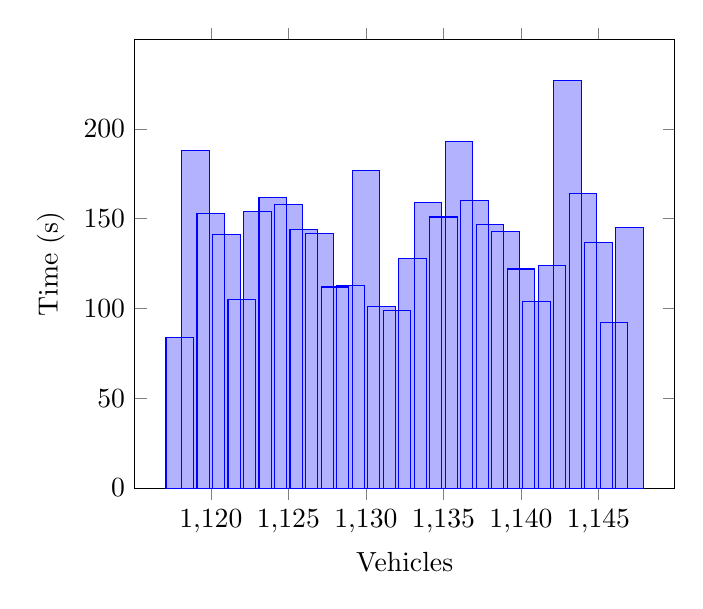
\begin{tikzpicture}
\begin{axis}[
legend style={anchor=west},
xlabel=Vehicles,
ylabel=Time (s),
ymin=0,
ybar,
]
\addplot coordinates {
(1144, 164)
(1122, 105)
(1123, 154)
(1124, 162)
(1135, 151)
(1139, 143)
(1138, 147)
(1133, 128)
(1132, 99)
(1131, 101)
(1130, 177)
(1137, 160)
(1136, 193)
(1134, 159)
(1127, 142)
(1142, 124)
(1143, 227)
(1140, 122)
(1141, 104)
(1146, 92)
(1147, 145)
(1145, 137)
(1126, 144)
(1129, 113)
(1128, 112)
(1120, 153)
(1121, 141)
(1125, 158)
(1119, 188)
(1118, 84)
};

\end{axis}
\end{tikzpicture}
\label{tik:time:100:71}
\caption{100 percent diving with GSC on route $71$}
\end{figure}
